%% SOURCE: experiments/010-kuzmin-tmi/scripts/positive_panel_selection.py -- gene table from results/positive_panel_fitness.csv, tier table from results/positive_panel_selected.csv
\section{The panel\secstatus{todo}}

Ten genes, all viable, all supported.

\begin{table}[H]
\centering
\begin{tabular}{llrrr}
\toprule
Block & Gene & single-mutant fitness & trigenic records & \% $\tau > +0.08$ \\
\midrule
1 & \texttt{YER059W} & 1.024 & 1097 & 16.3 \\
1 & \texttt{YGL060W} & 1.016 & 1321 & 3.6 \\
1 & \texttt{YGR121C} & 1.004 & 1413 & 9.6 \\
1 & \texttt{YHR003C} & 0.987 & 1356 & 6.6 \\
1 & \texttt{YPL181W} & 1.036 & 295  & 3.4 \\
\midrule
2 & \texttt{YDR423C} & 0.994 & 1049 & 9.6 \\
2 & \texttt{YHR204W} & 1.049 & 288  & 4.2 \\
2 & \texttt{YJR082C} & 0.976 & 796  & 2.0 \\
2 & \texttt{YKR028W} & 0.971 & 1323 & 14.7 \\
2 & \texttt{YLR258W} & 0.989 & 1114 & 5.1 \\
\bottomrule
\end{tabular}
\caption{Costanzo single-mutant fitness aggregated by mean across strain
backgrounds. No gene shows any disagreement between its KanMX and NatMX strains,
which is the check that \texttt{YJR060W} failed on the previous panel. The base
rate for $\tau > +0.08$ across the whole build is 5.4 percent.}
\end{table}

\subsection{Three tiers, and the contrast is the point\secstatus{todo}}

\begin{table}[H]
\centering
\begin{tabular}{llrrr}
\toprule
Tier & Triples & median predicted $\tau$ & range & median spread \\
\midrule
A, contains \texttt{YER059W}      & 6  & $+0.635$ & $+0.590$ to $+0.662$ & 0.081 \\
B, block 1 without \texttt{YER059W} & 4  & $+0.099$ & $+0.069$ to $+0.127$ & 0.446 \\
C, disjoint control               & 10 & $+0.029$ & $+0.011$ to $+0.044$ & 0.017 \\
\bottomrule
\end{tabular}
\caption{Predicted $\tau$ is the worst of three checkpoints; spread is the range
across them. All 20 triples are positive under all three checkpoints. The
training-label standard deviation is $0.0633$.}
\end{table}

The tiers are not three guesses of decreasing quality. They are a designed
contrast, and the reason for it is a property of the model rather than of the
selection. Across 6{,}934{,}927 complete five-gene blocks in this space the
positive confidence is concentrated in one clique: the best block sharing no gene
with it has a median predicted $\tau$ of $0.029$, under half the label standard
deviation, and no sixth gene extends the leading block above a median of
$0.024$. The distribution puts that in scale: the median block scores $-0.0005$
and the $99.99$th percentile $0.0196$, so the leading block's $0.607$ sits 31
times above the highest percentile the rest of the space reaches. Within that
block the six triples containing \texttt{YER059W} score $+0.590$ to $+0.662$ and
the four without it score $+0.069$ to $+0.127$.

So the model's positive claim is close to a single-gene claim, and the panel is
built to find that out. If measured $\tau$ orders A above B above C, the model is
ranking trigenic interactions. If A is high while B and C are indistinguishable,
it has learned one gene's marginal behavior and not interaction structure. If
none of the three separates, the ranking carries nothing at this scale. Every
outcome is readable, which a panel drawn only from tier A would not be.

Tier B is where the checkpoints disagree most, spreads of $0.34$ to $0.51$
against $0.08$ in tier A and $0.02$ in tier C. Removing \texttt{YER059W} from a
gene set the model is confident about does not lower its prediction so much as
destabilize it.

\begin{figure}[H]
\centering
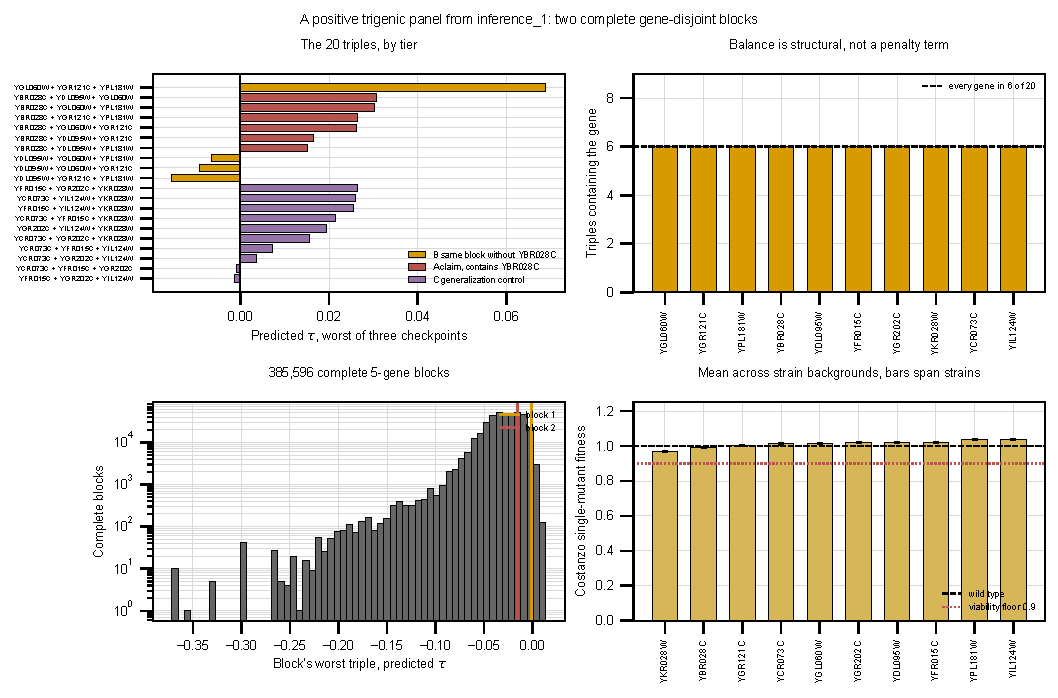
\includegraphics[width=\linewidth]{figures/positive_panel_selection.pdf}
\caption{The panel. Bars are the worst of three checkpoints, colored by tier.
Every gene sits in exactly 6 of the 20 triples. Both chosen blocks sit at the
extreme right of the distribution over all complete five-gene blocks. Every gene
is within 3 percent of wild-type single-mutant fitness. Generated by
\protect\file{experiments/010-kuzmin-tmi/scripts/positive_panel_selection.py}.}
\end{figure}
